\documentclass[11pt,a4paper]{article}
\usepackage[margin=25mm]{geometry}
\usepackage[T1]{fontenc}
\usepackage[utf8]{inputenc}
\usepackage{lmodern,microtype,amsmath,amssymb,booktabs,graphicx,array,longtable}
\usepackage[round,authoryear]{natbib}
\usepackage{caption,placeins,xcolor,fancyhdr}
\usepackage[colorlinks=true,linkcolor=teal,citecolor=teal,urlcolor=teal,breaklinks=true]{hyperref}
\usepackage{xurl}
\urlstyle{same}
\definecolor{teal}{HTML}{006D77}
\captionsetup{font=small,labelfont=bf}
\setlength{\parskip}{4pt}
\renewcommand{\floatpagefraction}{.8}
\renewcommand{\textfraction}{.1}
\renewcommand{\topfraction}{.9}
\setlength{\parindent}{12pt}
\setlength{\emergencystretch}{2em}
\pagestyle{fancy}\fancyhf{}\fancyhead[L]{\small Georgia's manganese frontier}\fancyhead[R]{\small Shivam Gupta}\fancyfoot[C]{\thepage}
\renewcommand{\headrulewidth}{0.3pt}
\title{\vspace{-14mm}\textbf{What Counts as Recovery?}\\[3mm]\large Manganese, Market Switching and Uneven Adjustment\\in Georgia, 2015--2025}
\author{Shivam Gupta\\\small Independent Researcher, India\\\small\href{mailto:shivam1720406@gmail.com}{shivam1720406@gmail.com}}
\date{16 October 2026}
\begin{document}
\maketitle\thispagestyle{empty}
\begin{abstract}
What does it mean for a commodity frontier to recover when its exports return but its earning capacity and market structure change? This paper examines Georgia's silicomanganese economy through annual destination-level trade records for 2015--2025 and monthly records for 2021--2025, situated in documentary research on the Chiatura--Zestafoni mining and smelting complex. It distinguishes physical throughput, gross export receipts and destination concentration. In 2024, export weight exceeded its 2022 level by 20.61\%, while nominal receipts remained 31.22\% lower. Yet the diagnosis depends on the benchmark: relative to 2019, 2024 weight and receipts were 0.66\% and 3.02\% higher. The rebound from 2023 increased destination concentration as T\"urkiye became the largest market. In 2025, receipts concentration fell by 65.41\%, even as weight fell by 25.24\% and receipts by 28.79\%. An exact two-group accounting decomposition attributes 65.85\% of that concentration decline to changes in the two largest 2024 destinations, T\"urkiye and the United States. Common-route decompositions also show why an aggregate unit-value decline cannot automatically be read as falling prices within continuing markets. Four established exporters also show lower unit receipts after 2022, although Georgia's decline is larger and composition remains unresolved. The contribution is a reproducible account of contrasting forms of adjustment at a Caucasian commodity frontier, rather than a causal estimate of trade policy or labour conflict. Recentring the frontier requires distinguishing the continued circulation of its commodity from the economic conditions under which that circulation persists.
\end{abstract}
\noindent\textbf{Keywords:} commodity frontiers; Georgia; manganese; export diversification; political ecology; trade measurement.\\
\textbf{JEL:} F14, Q32, R11.\\
\textbf{Research materials:} \url{https://github.com/shi1720/manganese-recovery-observatory}.

\section{Introduction}
A commodity can return to international circulation while the place that produces it remains in crisis. Conversely, a fall in dependence on a dominant export destination can look like successful diversification even when aggregate sales contract. Both possibilities matter for the interpretation of exhausted or contested commodity frontiers. A frontier is sustained through relations among extraction, processing, work, property and distant demand. None of these relations is adequately represented by a single export total.

Georgia's manganese economy offers a particularly revealing case. The Chiatura mining basin and Zestafoni ferroalloy industry connect a long-established Caucasian resource frontier to overseas steelmaking. The IOS COMFREE project places western Georgian manganese within the history of global industrialisation and peripheral resource incorporation \citep{ioscomfree}. This paper examines the frontier's contemporary adjustment, using national silicomanganese exports as an observable downstream trace of that relationship. It treats the national trade boundary and the local frontier as connected but distinct objects of inquiry.

The empirical puzzle is sharper than a contrast between growth and decline. Georgia's export weight rose strongly in 2024 after the 2023 contraction, but gross receipts remained below the 2021--2022 boom. T\"urkiye displaced the United States as the largest destination. In 2025 the destination portfolio became substantially less concentrated, yet both exported weight and receipts fell. These are different changes with different implications. A procurement analyst might welcome a broader range of destinations; a regional analyst concerned with the flow of gross receipts must also register contraction.

Existing accounts make the setting and the initial rebound visible. \citet{civil2024} reported renewed export activity alongside a further production suspension and uncertainty for workers. \citet{shamugia2025} discussed alternative markets as a reason to expect limited direct exposure to United States tariff changes. These observations preclude presenting either market switching or the coexistence of exports and crisis as a newly discovered phenomenon. The unresolved empirical task is to distinguish, over complete calendar years and on a reproducible basis, recovery in weight, recovery in receipts and the sources of measured diversification.

Three questions organise the analysis. First, how does the recovery diagnosis change with the outcome and the comparison year? Second, did the post-2023 reorientation reduce destination concentration, or replace one concentrated market structure with another? Third, when concentration eventually fell, how much of the change was associated with contraction in the largest markets rather than expansion elsewhere? We answer these questions with exact accounting decompositions, a full annual series, monthly consistency checks and transparent sensitivity exercises.

The findings qualify an undifferentiated recovery narrative. Relative to 2022, the 2024 quantity rebound coexisted with a receipts shortfall of US\$141.43 million. Relative to 2019, the same year was close to parity in weight and modestly ahead in nominal receipts. Concentration rose between 2023 and 2024, while its sharp decline in 2025 accompanied a US\$89.70 million receipts contraction. Approximately two-thirds of that decline in concentration is assigned to changes in T\"urkiye and United States sales by an explicitly defined two-group decomposition. The remaining destinations expanded their combined receipts, but insufficiently to replace losses in those two markets.

The paper contributes a new empirical reconstruction and an implementable measurement workflow. Its methods are established accounting devices. Its case-specific contribution is to show that the sequence from boom to contraction, concentrated rebound and contracting diversification cannot be described faithfully as one continuous restoration of market security. This is a bounded contribution to the study of commodity frontiers and uneven adjustment; the evidence does not establish household welfare, environmental improvement or the effects of a particular policy.

\section{Commodity frontiers, dependence and the meaning of recovery}
\subsection{Recentring a continuing frontier}
The commodity-frontier approach connects the incorporation of land and labour into global accumulation with place-specific degradation, adaptation and resistance \citep{beckert2021}. It directs attention to the social and ecological relations that enable commodity circulation. Here, recovery is therefore an analytical question about the conditions of continued incorporation, rather than a synonym for a positive annual export growth rate.

The historical importance of manganese does not settle the present distribution of adjustment costs. A material can remain necessary for industrial production while individual producing places lose sales or bargaining room. Work on criticality distinguishes supply risk, vulnerability and environmental implications rather than reducing them to one universal label \citep{graedel2015}. \citet{nassar2020} explicitly evaluate supply risk from the perspective of United States manufacturing. Our question begins at the exporting end of the relationship. It asks which monetary and geographical conditions accompany continued outward movement of a specific processed commodity. Silicomanganese exports should not be conflated with battery-grade manganese products or with all uses of the element.

\citet{mataradze2025} considers Chiatura's industrial constraints and strategies for higher-value production. This paper addresses a different margin: observed sales of the existing silicomanganese product across destinations. It makes no claim that market switching achieves technological upgrading. Even a rise in dollars per kilogram would not, by itself, establish an improvement in domestic value added or the share received by labour.

\subsection{Destination breadth and the scale of circulation}
The relationship between foreign trade and asymmetric dependence has a long history \citep{hirschman1945}. A country selling into several markets need not be secure against the loss of its largest buyers. Nor does a smaller share for one buyer reveal whether other buyers have expanded enough to preserve total receipts. Relative shares must be read alongside their denominators.

The export-margin literature likewise distinguishes establishing relationships from maintaining and deepening them. \citet{besedes2011} demonstrate why relationship survival matters for sustained export growth. In our application, a destination absent in one comparison year but present in the next is an observed route entry; it is not necessarily a first-ever market discovery. A positive destination count measures geographical reach, while the Herfindahl--Hirschman index (HHI) measures the unequal distribution of activity within that reach. Neither is a measure of the diversity of domestic production.

We consequently use three separate outcomes: \emph{throughput}, the reported mass crossing the export boundary; \emph{gross receipts}, the nominal dollar value of those exports; and \emph{destination structure}, the distribution of either measure across markets. We do not combine them into a composite recovery score. Such aggregation would hide a normative decision about how much lost revenue should be offset by a broader portfolio of destinations.

\subsection{Local conditions and the limits of the customs boundary}
Chiatura's continuing crisis is already the subject of substantial research. \citet{eristavi2026} relates the town's harms to postsocialist restructuring and state--corporate relations, emphasising the institutions that permit harmful economic activity. \citet{hrw2019} documents mining safety problems in the context of deregulation. Contemporary labour organisations also make claims about working conditions and compensation that cannot be reduced to interruptions of export supply \citep{sjc2023b}.

These accounts establish why a local recovery question exceeds customs statistics. This paper adds evidence about outward trade, rather than treating trade records as a substitute for local testimony. A decline in exports does not demonstrate ecological restoration; damage can persist after extraction slows. An increase in receipts does not demonstrate improved wages, compensation or safety. A broader destination portfolio does not establish greater local participation in decisions over land or work. These distinctions are constitutive of the research design, not qualifications added after interpreting the results.

\section{Sources, scope and research design}
\subsection{Trade records}
The primary source is UN Comtrade, queried for Georgia-reported exports of HS 720230, ferro-silico-manganese, for 2015--2025 annually and 2021--2025 monthly \citep{comtrade2026}. Each query selects one reporter, one period, one commodity, total partner-2, total customs procedure and total transport mode, and retrieves all destination partners. World aggregates are retained for validation and excluded from partner sums. The original reported HS edition is preserved in the raw responses; the commodity selection remains the six-digit 720230 category throughout the window.

The annual Georgian sample contains 317 positive partner-year records and eleven World records. The monthly sample contains 675 positive partner-month records across sixty complete reporter-period queries. Each response is below the public endpoint's 500-record ceiling. Raw JSON, complete query URLs, record counts and SHA-256 checksums are archived with the code. The retrieval session is dated 16 October 2026. The analysis is exploratory and retrospective; the repository protocol records that initial annual data were inspected before the comparisons were finalised.

We use reported net weight in kilograms, $q_{jt}$, and primary trade value in current United States dollars, $v_{jt}$. The Georgian quantity unit is kilogram and the net-weight estimation flag is false. Supplementary quantity and net weight agree in all monthly records and in annual records for 2016--2025. In 2015, they differ for two destinations and their World aggregate, by a combined 287,000 kg. Analysis consistently uses net weight; the cross-field discrepancies are preserved in the validation output. These checks support consistency within this extraction; they do not prove that national declarations are error-free. UN Comtrade guidance cautions that null or zero quantity can indicate missing measurement \citep{unquantity}. No such records enter the positive Georgian series analysed here.

Wholly missing reporter-periods are never filled with zero. Within a retrieved period whose partner totals match World, a destination with no positive record is treated as zero recorded trade for the purpose of accounting. This convention describes the database's coverage of the selected commodity and dimensions. It does not prove the absence of informal trade, misclassification or indirect shipment through another country.

\subsection{The place observed by the data}
The statistical object is Georgia's silicomanganese export economy. It is not the output of a single mine, firm or municipality. Ore extraction, concentration, alloy production and customs shipment are separate stages. Stock releases, imported inputs, other producers and shipment timing can disconnect national exports from current Chiatura extraction. Consequently, the empirical estimates describe adjustment at the national commodity boundary, situated in the documented Chiatura--Zestafoni relationship. They do not allocate a measured export loss to particular workers or villages.

We also retrieve World export records for South Africa, India, Malaysia and Norway for 2019--2025 as an external unit-receipts check. These four established suppliers were selected from the industry review before inspecting their export series. Only the complete, non-estimated 2022, 2024 and 2025 weights enter the displayed comparison; missing or estimated weights in other years remain visible in the archive. The comparator group is purposive, not a representative sample of world producers.

We retain United States annual imports of the same six-digit product as a separate diagnostic. They are not used to replace Georgia's declarations. For example, in 2023 Georgian exports to the United States are recorded as US\$68.69 million, while United States imports from Georgia are US\$62.30 million. There are also important differences between supplementary quantity and the net-weight field in the United States series. Appendix~\ref{app:mirror} reports these discrepancies without assigning an unsupported single explanation. General guidance on bilateral asymmetries makes clear why mirror flows should not be silently averaged \citep{unmirror}.

\subsection{Documentary contextualisation}
The documentary corpus was assembled to establish the commodity chain, locate the trade chronology and identify competing interpretations. It includes the IOS project description, research on Georgian extractive institutions, a Georgian mining article with an English abstract, local labour advocacy, contemporary reporting and a USITC industry review. Each performs a different evidentiary role. Company explanations and advocacy claims are attributed; neither is treated as a controlled causal test.

The USITC review places the February 2023 mine suspension before the June labour dispute and describes the connection from Chiatura ore to Zestafoni production \citep{usitc2024}. Reporting in November 2024 describes a further announced suspension, falling market prices and disputes over damage to homes and orchards \citep{civil2024}. These records establish that market conditions and local conflict overlap. They do not identify the contribution of either to annual export changes. In particular, the sequence does not justify treating worker protest as the initial cause of the 2023 contraction.

\section{Accounting methods}
\subsection{Totals, unit receipts and concentration}
For destinations $j$ in year $t$, define
\begin{equation}
 V_t=\sum_j v_{jt},\qquad Q_t=\sum_j q_{jt},\qquad P_t=V_t/Q_t.
\end{equation}
$P_t$ is aggregate \emph{unit export receipts}, not a transaction-price index. It changes with market composition, grades, contract conditions and prices. We report it in USD/kg; weights in the tables are thousand metric tonnes and values are million current USD.

With $s^V_{jt}=v_{jt}/V_t$ and $s^Q_{jt}=q_{jt}/Q_t$, the concentration measures are
\begin{equation}
 H^V_t=\sum_j(s^V_{jt})^2,\qquad H^Q_t=\sum_j(s^Q_{jt})^2.
\end{equation}
The inverse $1/H^V_t$ gives the effective number of equally sized destinations with the same concentration. Value and weight HHI answer different questions. Their disagreement can reflect destination differences in unit receipts and should not be resolved by choosing whichever supports the preferred narrative.

\subsection{Decomposing changes in receipts}
We use the classical symmetric midpoint identity, associated with Bennet-type additive indicators \citep{bennet1920}:
\begin{equation}\label{eq:aggregate}
 V_1-V_0=\underbrace{\frac{P_1+P_0}{2}(Q_1-Q_0)}_{\text{aggregate weight component}}
 +\underbrace{\frac{Q_1+Q_0}{2}(P_1-P_0)}_{\text{aggregate unit-receipts component}}.
\end{equation}
It is an exact identity, not an estimate of a demand or supply response. The components describe the observed endpoints symmetrically, avoiding a choice between applying only initial or only final unit receipts.

The aggregate component mixes within-destination changes with market reallocation. We therefore also decompose receipts over destinations active at both endpoints, $C$, observed entrants, $E$, and observed exits, $X$:
\begin{align}\label{eq:routes}
 \Delta V={}&\sum_{j\in C}\frac{p_{j1}+p_{j0}}{2}(q_{j1}-q_{j0})
 +\sum_{j\in C}\frac{q_{j1}+q_{j0}}{2}(p_{j1}-p_{j0})\nonumber\\
 &+\sum_{j\in E}v_{j1}-\sum_{j\in X}v_{j0},\qquad p_{jt}=v_{jt}/q_{jt}.
\end{align}
No price is invented for an inactive route. Entry and exit remain separate monetary terms. The second term is still a within-route \emph{unit-receipts} component: product grades can vary even within a destination. Appendix~\ref{app:proof} verifies both identities algebraically.

\subsection{Attributing a change in concentration}
For 2024--2025, let $A$ be the two largest 2024 markets by receipts, T\"urkiye and the United States, and let $B$ contain every other destination in the union of endpoint supports. Write $H(A_i,B_k)$ for HHI computed using group $A$'s receipts from endpoint $i$ and group $B$'s receipts from endpoint $k$. A two-group Shapley decomposition averages both update orders \citep{shapley1953}:
\begin{align}
 \phi_A={1\over2}\{H(A_1,B_0)-H(A_0,B_0)\}
 +{1\over2}\{H(A_1,B_1)-H(A_0,B_1)\},\\
 \phi_B=\Delta H-\phi_A.
\end{align}
Each hybrid state's denominator is recalculated. Holding baseline shares fixed would fail to capture HHI's nonlinear response to changing totals. This decomposition is order-symmetric for the declared grouping, but group choice is substantive and was made after inspecting the data. It is not a unique causal allocation of diversification. We report the monetary changes of both groups so that the attribution is interpretable.

\subsection{Validation and sensitivity}
The analysis checks response completeness, uniqueness of record keys, units, estimation flags, partner-to-World sums and monthly-to-annual sums. A separate standard-library program recomputes headline results using decimal arithmetic directly from raw JSON. Randomised numerical tests verify the accounting identities; they evaluate the implementation, not an economic hypothesis.

All annual benchmarks before the 2024 and 2025 endpoints are reported in the machine-readable outputs. The paper highlights 2019 as a pre-pandemic benchmark alongside the 2022 boom and the 2023 trough. Deterministic error screens allow each positive observation's value or weight to move within a stated proportional range. These are sensitivity ranges, not confidence intervals. Administrative totals do not furnish a calibrated sampling distribution for the measurement errors of interest here.

\section{Results}
\subsection{A rebound whose meaning changes with the benchmark}
Table~\ref{tab:annual} and Figure~\ref{fig:recovery} show the annual path. Receipts reach their maximum in 2021, while aggregate unit receipts peak in 2022. Export weight peaks in 2021 as well. Thus 2022 is a high-unit-receipt benchmark, not an unambiguously normal level of throughput or income.

\begin{table}[htbp]\centering\small
\caption{Georgia's silicomanganese exports: complete annual series.}\label{tab:annual}
\begin{tabular}{rrrrrrr}\toprule
Year & Receipts & Weight & USD/kg & Value HHI & Weight HHI & Destinations\\
 & (US\$m) & (kt) & & & & \\\midrule
2015 &183.66&205.50&0.894&0.222&0.206&28\\
2016 &168.24&227.93&0.738&0.188&0.179&36\\
2017 &300.21&275.69&1.089&0.300&0.289&33\\
2018 &345.97&291.84&1.185&0.321&0.309&27\\
2019 &302.44&273.88&1.104&0.301&0.284&26\\
2020 &247.20&250.54&0.987&0.278&0.266&28\\
2021 &477.07&299.09&1.595&0.274&0.262&32\\
2022 &453.01&228.58&1.982&0.339&0.290&26\\
2023 &178.52&155.95&1.145&0.262&0.250&24\\
2024 &311.58&275.69&1.130&0.305&0.298&30\\
2025 &221.88&206.10&1.077&0.106&0.105&27\\\bottomrule
\end{tabular}
\caption*{Source: author's calculations from UN Comtrade. kt = thousand metric tonnes; US\$m = million current USD. Destinations count positive recorded partner flows.}
\end{table}

\begin{figure}[htbp]\centering
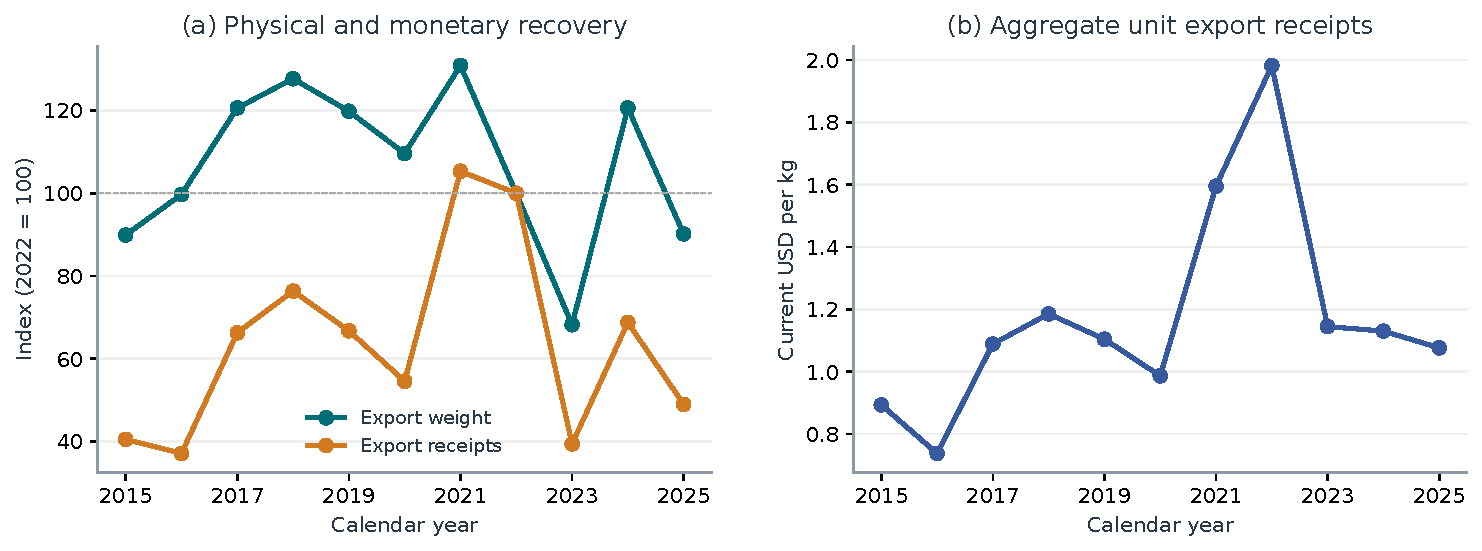
\includegraphics[width=\linewidth]{../figures/01_recovery.pdf}
\caption{Recovery depends on the outcome. Left: export weight and receipts indexed to 2022. Right: aggregate unit receipts. All observations are annual totals; current USD are not inflation-adjusted. Source: author's calculations from UN Comtrade.}\label{fig:recovery}
\end{figure}

From 2022 to 2023, weight falls by 31.78\% and receipts by 60.59\%. The 2024 rebound is substantial: weight rises by 76.78\% and receipts by 74.53\% relative to the trough. Nevertheless, comparison with 2022 yields 20.61\% more weight and 31.22\% fewer receipts. The aggregate unit-receipts ratio is 42.97\% lower. Equation~\ref{eq:aggregate} allocates the US\$141.43 million receipts shortfall to a positive US\$73.31 million weight component and a negative US\$214.74 million aggregate unit-receipts component.

That result does not establish a long-run decline relative to every earlier year. Relative to 2019, 2024 weight is 0.66\% higher, receipts 3.02\% higher and unit receipts 2.34\% higher. Relative to 2021, however, both 2024 weight and receipts remain lower. The appropriate statement is therefore that physical recovery from the trough did not restore boom-period receipts. Calling 2024 an unprecedented collapse in earning conditions would be equally misleading. Table~\ref{tab:benchmarks} makes the benchmark dependence explicit.

\begin{table}[htbp]\centering\small
\caption{Contrasting recovery diagnoses: percentage changes.}\label{tab:benchmarks}
\begin{tabular}{lrrrrr}\toprule
Comparison & Receipts & Weight & USD/kg & Value HHI & Weight HHI\\\midrule
2019--2024 &3.02&0.66&2.34&1.47&4.76\\
2022--2024 &$-31.22$&20.61&$-42.97$&$-10.00$&2.50\\
2023--2024 &74.53&76.78&$-1.27$&16.46&18.85\\
2024--2025 &$-28.79$&$-25.24$&$-4.75$&$-65.41$&$-64.69$\\
2022--2025 &$-51.02$&$-9.83$&$-45.68$&$-68.87$&$-63.81$\\\bottomrule
\end{tabular}
\caption*{Each entry is $100(x_1/x_0-1)$. A negative HHI change means lower destination concentration.}
\end{table}

\subsection{Market switching concentrated the 2024 rebound}
The rebound reconstitutes the destination geography rather than restoring the earlier one (Figure~\ref{fig:destinations}). Between 2022 and 2024, recorded receipts from the United States fall from US\$232.97 million to US\$89.70 million. Recorded exports to Russia, worth US\$107.79 million in 2022, have no positive record in 2024. T\"urkiye grows from US\$55.67 million to US\$144.46 million and becomes the largest destination, accounting for 46.37\% of receipts and 46.84\% of weight in 2024.

\begin{figure}[htbp]\centering
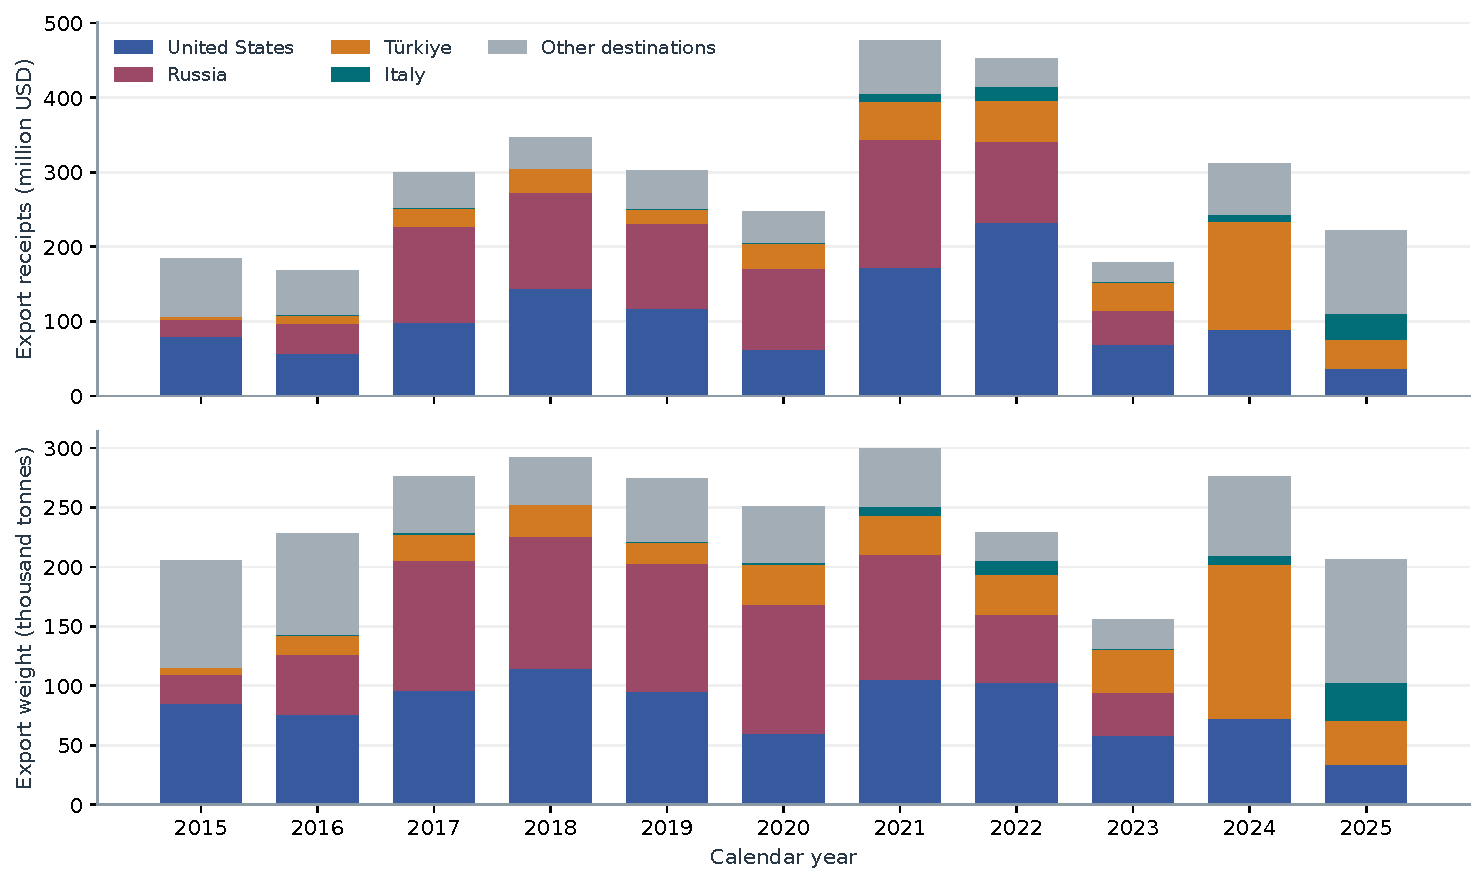
\includegraphics[width=\linewidth]{../figures/02_destinations.pdf}
\caption{The geography of adjustment in receipts and physical weight. Fixed destination groups preserve comparability across the series. ``Other destinations'' includes all positive partners outside the four separately shown. Source: author's calculations from UN Comtrade.}\label{fig:destinations}
\end{figure}

This is market switching with renewed concentration. From 2023 to 2024, value HHI rises from 0.262 to 0.305 and weight HHI from 0.250 to 0.298. The effective number of destinations by value falls from 3.82 to 3.28 even as the count of positive destinations rises from 24 to 30. The six additional recorded destinations therefore do not constitute a less concentrated distribution of sales. Most activity remains concentrated in a few outlets.

The longer comparison produces a second measurement warning. Relative to 2022, value HHI is 10.00\% lower in 2024, but weight HHI is 2.50\% higher. In monetary shares the portfolio appears somewhat less concentrated; in physical shares it appears slightly more concentrated. The difference is not an error in HHI. Destination-specific unit receipts weight the same market geography differently. A claim of ``diversification'' needs to specify the ledger and period it refers to.

\subsection{Lower concentration in 2025 accompanied contraction}
The 2025 structure is markedly broader by both measures (Figure~\ref{fig:concentration}). Value HHI falls to 0.106, a 65.41\% decrease, and weight HHI falls by 64.69\%. The effective number of destinations rises to 9.47, although the number of positive destinations falls from 30 to 27. Broader economic distribution and the count of destinations again move in opposite directions.

\begin{figure}[htbp]\centering
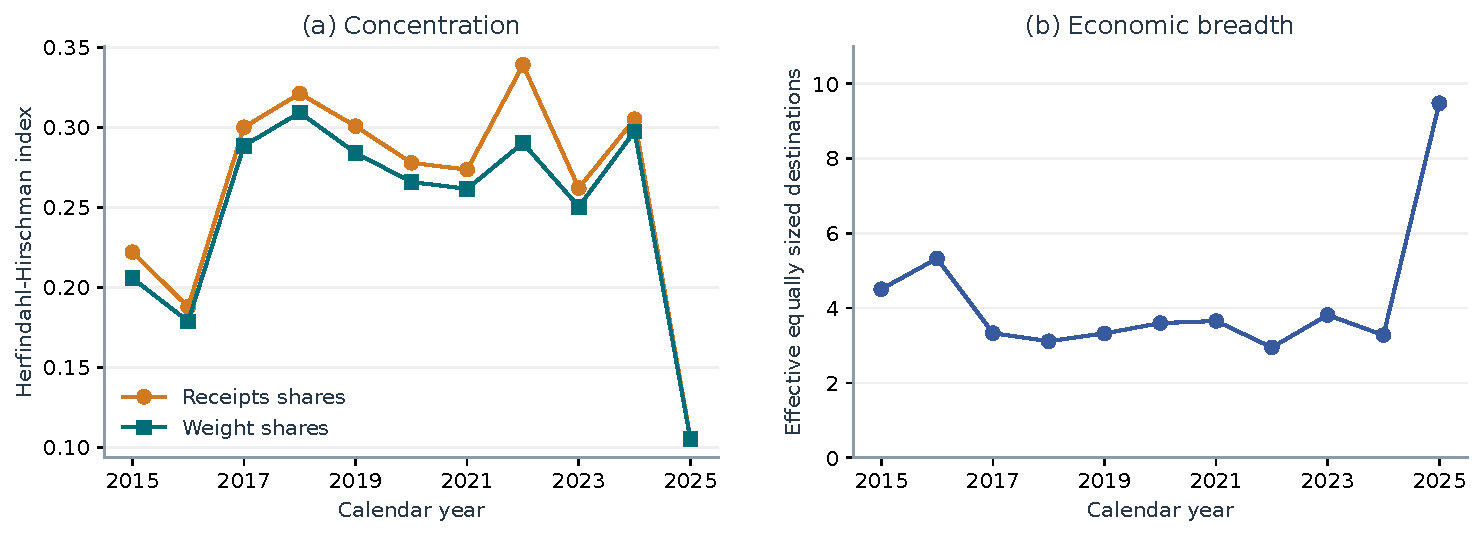
\includegraphics[width=\linewidth]{../figures/03_concentration.pdf}
\caption{Destination concentration and effective breadth. HHI is reported on its unnormalised 0--1 scale. The inverse of value HHI measures equivalent equally sized markets, rather than the observed count of destinations. Source: author's calculations from UN Comtrade.}\label{fig:concentration}
\end{figure}

Yet 2025 also brings a 25.24\% decline in export weight and a 28.79\% decline in receipts. T\"urkiye's receipts fall by US\$105.37 million and United States receipts by US\$52.98 million. Together the two markets lose US\$158.35 million. All other destinations together gain US\$68.65 million, leaving the total US\$89.70 million lower. Italy, Greece, the Netherlands and Spain are among the expanding destinations. The change therefore contains real growth elsewhere as well as contraction in the previously largest markets.

The two-group decomposition assigns $-0.13146$ HHI points to the T\"urkiye--United States group and $-0.06816$ to the remaining destinations, summing to the observed $-0.19962$. Changes in the two largest markets account for 65.85\% of the measured concentration decline under this grouping. This is not a finding that all diversification was caused by loss. It shows that expanding secondary markets and shrinking dominant markets jointly produced a broader portfolio whose total receipts were substantially smaller.

\subsection{Aggregate unit receipts can conceal a different continuing-market pattern}
Table~\ref{tab:decomp} and Figure~\ref{fig:decomp} report Equation~\ref{eq:routes}. For 2023--2024, continuing routes contribute US\$154.86 million through weight changes and US\$11.42 million through unit-receipts changes. Entries add US\$13.11 million and exits subtract US\$46.34 million. Their sum is the observed US\$133.05 million rebound.

\begin{table}[htbp]\centering\small
\caption{Exact receipts decomposition by route status, million current USD.}\label{tab:decomp}
\begin{tabular}{lrrrrr}\toprule
Comparison & Common-route & Common-route & Entry & Exit & Total\\
 & weight & unit receipts & & & \\\midrule
2022--2023 &$-123.08$&$-150.74$&10.51&$-11.18$&$-274.49$\\
2022--2024 &89.99&$-152.25$&29.57&$-108.74$&$-141.43$\\
2023--2024 &154.86&11.42&13.11&$-46.34$&133.05\\
2024--2025 &$-80.18$&$-14.08$&33.26&$-28.70$&$-89.70$\\\bottomrule
\end{tabular}
\caption*{Common routes have positive weight at both endpoints. Entry and exit refer only to the endpoint comparison, not first-ever appearance or permanent disappearance. Rounding can affect displayed sums by US\$0.01 million.}
\end{table}

\begin{figure}[htbp]\centering
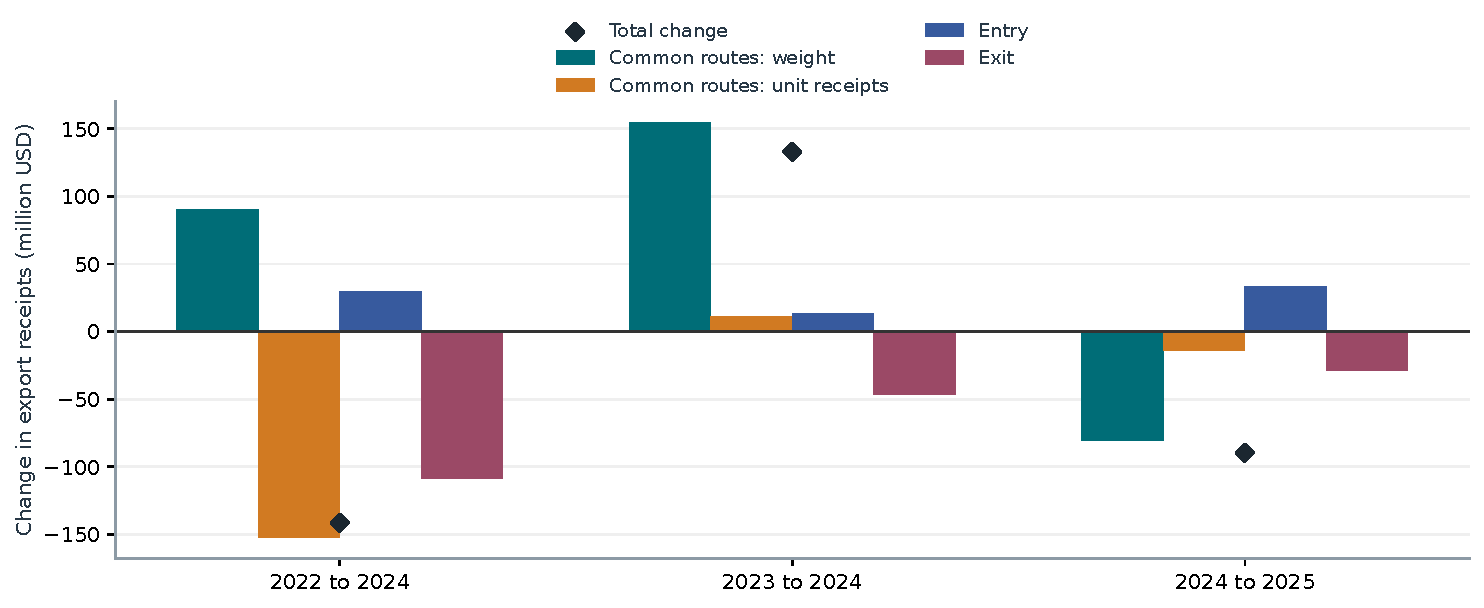
\includegraphics[width=\linewidth]{../figures/04_decomposition.pdf}
\caption{Different adjustments underlie the rebound and subsequent contraction. Bars show route-level midpoint components and entry/exit terms; diamonds show their total. These are accounting contributions, not causal effects. Source: author's calculations from UN Comtrade.}\label{fig:decomp}
\end{figure}

The positive continuing-route unit-receipts contribution in 2023--2024 coexists with a negative aggregate unit-receipts component of US\$3.15 million in Equation~\ref{eq:aggregate}. The apparent contradiction is informative: reallocation and route turnover change the average dollars per kilogram even when the symmetric continuing-route component is positive. It would be incorrect to equate the 1.27\% aggregate decline with a general fall in prices in all continuing markets.

For 2022--2024, the continuing-route unit-receipts component is strongly negative, at US\$152.25 million. Observed exits, dominated by Russia, subtract another US\$108.74 million, while continuing-route weight changes and entries partly offset them. The result is consistent with a substantial loss of boom-period unit receipts, but it also identifies the independent importance of route turnover. For 2024--2025, continuing-route weight changes dominate the receipts decline; new route receipts cannot offset the combined contraction and exit terms.

\subsection{Monthly timing and robustness}
Figure~\ref{fig:monthly} retains monthly variability rather than interpolating a smooth recovery path through annual endpoints. It marks February 2023 and November 2024, the documented suspension episodes, as chronological reference points. Shipment timing, stock release and contracts can shift the relationship between these dates and customs flows. The figure is therefore not an event study and the lines do not identify a treatment onset.

\begin{figure}[htbp]\centering
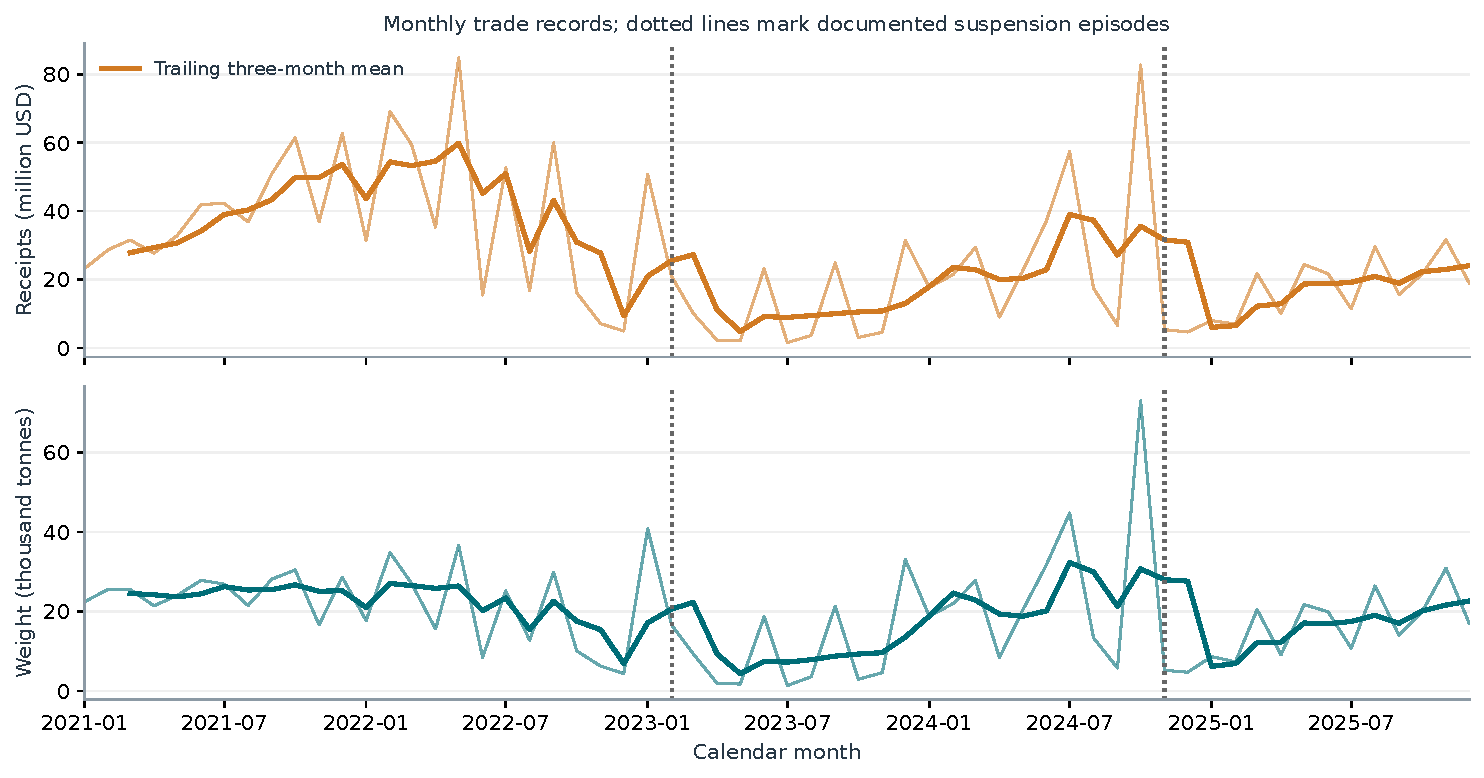
\includegraphics[width=\linewidth]{../figures/05_monthly.pdf}
\caption{Monthly export receipts and weight, January 2021--December 2025. Thin lines are monthly observations; thicker lines are trailing three-month means. Dotted dates locate documented suspension episodes; they do not identify causal effects on shipments. Source: UN Comtrade; documentary chronology in \citet{usitc2024,civil2024}.}\label{fig:monthly}
\end{figure}

The main directional claims survive a conservative measurement screen. If each positive observation's value and weight can vary independently by up to 5\%, the 2022--2024 weight ratio remains between 1.091 and 1.333 and the receipts ratio between 0.622 and 0.760. The 2024--2025 ratios remain between 0.676 and 0.826 for weight and between 0.644 and 0.787 for receipts. A conservative bound for the HHI ratio, derived in Appendix~\ref{app:sensitivity}, places the 2025-to-2024 value HHI ratio below 0.517 even under these perturbations. The decline in concentration is therefore too large to be reversed by that screen.

These bounds do not imply that every component or small difference is equally robust. In particular, the 2.50\% increase in weight HHI between 2022 and 2024 and the near-parity comparison with 2019 warrant modest interpretation. Nor does the screen account for systematic product misclassification or missing informal trade. It states what follows under the declared proportional-error model, rather than estimating the probability that the declarations are correct.

\subsection{An external check on the boom reversal}
The external exporters also experience lower unit receipts after 2022 (Table~\ref{tab:reference}). Between 2022 and 2024 their declines range from 18.34\% in South Africa to 34.39\% in Malaysia, compared with 42.97\% in Georgia. The general direction is therefore shared, but Georgia's decline is larger than that of every member of this comparator group. In 2025 Georgia's unit receipts remain 45.68\% below 2022; the corresponding comparator declines range from 11.05\% to 36.98\%.

\begin{table}[htbp]\centering\small
\caption{Unit export receipts in Georgia and four established exporters.}\label{tab:reference}
\begin{tabular}{lrrrrr}\toprule
Exporter & 2022 & 2024 & 2025 & 2022--2024 & 2022--2025\\
 & \multicolumn{3}{c}{Current USD/kg} & \multicolumn{2}{c}{Change (\%)}\\\midrule
South Africa &1.227&1.002&1.091&$-18.34$&$-11.05$\\
India &1.299&0.911&0.905&$-29.90$&$-30.32$\\
Malaysia &1.456&0.955&0.918&$-34.39$&$-36.98$\\
Norway &1.456&1.166&1.089&$-19.93$&$-25.24$\\
Georgia &1.982&1.130&1.077&$-42.97$&$-45.68$\\\bottomrule
\end{tabular}
\caption*{Source: each exporter's own UN Comtrade World record, HS 720230. These displayed weights are positive and not flagged as estimated. The same product code does not ensure identical grade, contract or destination composition.}
\end{table}

This check prevents two overinterpretations. Georgia's receipts decline cannot be presented as wholly detached from a wider commodity cycle. Its larger percentage decline also cannot be interpreted as a causal measure of peripheral disadvantage: Georgia begins from markedly higher unit receipts in 2022, and differences in grade, contracts and market composition are unresolved. The evidence supports a shared direction of adjustment with unequal observed magnitudes, rather than a quality-adjusted international price penalty. A four-exporter comparison is insufficient to identify a global benchmark price.

\section{Discussion: the frontier persists through uneven adjustment}
\subsection{Three scales of recovery}
The evidence distinguishes three scales often compressed into a single recovery story. At the commodity boundary, more physical material can circulate. At the national receipts boundary, the same activity can deliver fewer dollars than during a boom. At the regional social and ecological boundary, neither change identifies the distribution of work, compensation or damage. The first two are measured here; the third is situated through existing research and remains an open empirical task.

This separation changes the interpretation of the frontier's persistence. Georgia's 2024 silicomanganese exports do not describe simple abandonment. Substantial circulation resumes through a reconfigured set of destinations. But concentrated reorientation is followed in 2025 by a broader and smaller receipts portfolio. A frontier can remain integrated into international production through such sequences without returning to its previous monetary conditions. The meaningful question is the terms on which incorporation continues.

It would be equally mistaken to infer that every change after 2022 represents deterioration from a sustainable norm. The 2019 comparison demonstrates why a high-unit-receipt benchmark can magnify the appearance of a persistent discount. The paper's claim is narrower and more useful: physically similar export activity can occupy substantially different monetary positions, and its assessment depends on the benchmark. This is a reason to display the full trajectory, rather than select one endpoint as an unquestioned recovery target.

\subsection{Reading local conflict against global adjustment}
The trade sequence makes space for local histories without explaining them away. Domestic disputes over work and damaged property cannot be treated as friction around an otherwise self-contained export process. At the same time, a national customs series cannot establish how overseas market changes translated into a specific management decision. The available documents identify competing explanations and overlapping pressures; they do not supply firm accounts, transaction contracts or a counterfactual wage path.

A stronger future causal study would need linked producer sales, inventories, input sourcing, employment and compensation records. Those data would distinguish reduced current extraction from stock disposal, and gross receipts from local income. For present purposes, the defensible inference is that export-led indicators provide an incomplete account of frontier recovery. They can establish continued commodity circulation and its market geography; they cannot certify the restoration of the social relations that sustain a place.

\subsection{Practical applications}
The results have a concrete use in trade monitoring and regional economic assessment. A dashboard that reports only annual export growth would label 2024 a strong recovery. One that reports only lower concentration would label 2025 a diversification success. A companion observatory therefore displays receipts, weight, unit receipts, value and weight HHI, and the contributions of contracting dominant markets together. Its rules are transparent, require no predictive model and can be applied to another commodity once its units and statistical boundary have been checked.

Potential users include commodity exporters assessing destination exposure, development institutions monitoring resource-dependent regions, and buyers assessing continuity in supplier economies. The commercial opportunity is an auditable analytics service around a documented decision problem, not a demonstrated willingness to pay or a proprietary discovery in concentration mathematics. Existing shipment-data products already cover trade flows. The proposed implementation's useful distinction is to keep recovery claims, benchmarks and accounting contributions inspectable. The present study validates calculations and their interpretation on this case; it does not validate a forecasting product.

\section{Limitations}
This is a single-commodity national case with an eleven-year annual window and five years of monthly detail. It cannot establish the prevalence of the observed sequence across Eurasian resource economies. The commodity was selected for its regional and documentary fit, and the analysis is exploratory. The full comparison grid and code reduce selective reporting but do not turn the design into a preregistered confirmatory study.

All receipts are nominal United States dollars. They are gross border values, not profits, local purchasing power, value added or tax receipts. Unit receipts mix price, quality, contract and composition effects. The midpoint decompositions are exact for the selected records but not structural economic models. Destination records may describe immediate rather than ultimate markets, so country diversification need not imply diversification of firms, beneficial ownership or final steel demand.

Finally, chronology and co-movement are insufficient for causal attribution. We do not estimate the effect of protests, sanctions, tariffs, special management or ownership. We do not assume that a fall in national exports is an environmental gain, or that a critical-mineral designation protects a particular mining community. The paper is conclusive about the recorded accounting contrasts and deliberately limited about the mechanisms beyond them.

\section{Conclusion}
Georgia's manganese frontier experienced several different adjustments after the boom. The 2024 rebound restored physical exports relative to 2022 while leaving a substantial receipts shortfall; relative to 2019 it was close to nominal parity. That rebound increased destination concentration compared with the 2023 trough. The major decline in concentration arrived in 2025, alongside falling weight and receipts, and was substantially associated with shrinking sales to the two previously largest markets.

These results make a specific contribution to recentering the margins of the world economy. They show how a peripheral commodity economy can remain active in global circulation while its monetary and geographical conditions change in divergent directions. A defensible account of recovery must name the outcome, comparison period and place to which it refers. Open accounting cannot replace local history, but it can prevent a national export headline from standing in for it.

\section*{Data and code availability}
The companion repository contains the raw API responses, query manifest, analytical code, tests, independent decimal verification, derived tables, vector figures, manuscript source and an offline observatory. Code is released under the MIT licence; the manuscript and original figures under CC BY 4.0. UN Comtrade data remain subject to their source terms and are attributed separately. The repository's literature review records the nearest identified antecedents and the scope of the novelty claim. No claim of exhaustive absence of prior research is made.

\FloatBarrier
\bibliographystyle{plainnat}
\bibliography{references}
\clearpage
\appendix
\section{Reproducibility and data checks}\label{app:validation}
The analysis queries 22 annual reporter-periods: eleven Georgian export years and eleven United States import years. It also queries sixty Georgian export months and 28 World export records for the external comparator group, for 110 archived responses in total. The Georgian annual partner counts sum to 317, and the monthly sample contains 675 positive partner-month records and sixty World records. All partner-year weights and values are positive; no Georgian net-weight record is flagged as estimated. The annual partner sums match World to within US\$0.01 and 0.01 kg, allowing the precision of the response. Monthly partner sums also match World. Annual and summed monthly receipts differ by no more than US\$0.002. Summed monthly weight exceeds the annual declaration by 171.5 kg in 2022 (0.000075\%); the other four years match. Annual results use annual declarations, and monthly figures use monthly records without forcing reconciliation. The tests preserve this observed discrepancy. Final counts and maximum residuals are written to \texttt{data/derived/validation\_summary.json}.

The analysis can be reproduced from the archived snapshot without network calls:
\begin{verbatim}
python3 -m pip install -r requirements.txt
python3 src/analyze.py
python3 src/reference.py
python3 src/verify_independently.py
python3 -m unittest discover -s tests -v
python3 src/figures.py
python3 src/dashboard.py
cd paper
tectonic manuscript.tex
\end{verbatim}
The test suite includes 1,000 random midpoint-identity cases and 1,000 random concentration-attribution cases, as well as source and aggregation checks. The independent verifier uses the standard library and decimal arithmetic and checks primary percentage changes to within $10^{-6}$ percentage point. These are numerical validation tolerances; they should not be interpreted as the accuracy of the underlying declarations.

\section{Mirror records and measurement boundaries}\label{app:mirror}
Table~\ref{tab:mirror} preserves selected mirror discrepancies. Georgia's figures use its export net weight. The United States columns display supplementary quantity and net weight separately. We do not infer identical measurement bases from a shared kilogram label. For 2024 those United States fields coincide, whereas in 2022 and 2023 they differ materially. No conversion factor is fitted to force a match.

\begin{table}[htbp]\centering\small
\caption{The Georgia--United States route in the two reporting systems.}\label{tab:mirror}
\begin{tabular}{rrrrrr}\toprule
Year & Georgia value & Georgia weight & US value & US quantity & US net weight\\
 & (US\$m) & (kt) & (US\$m) & (million kg) & (million kg)\\\midrule
2021 &172.34&105.09&131.86&87.83&64.71\\
2022 &232.97&102.54&260.83&113.95&82.25\\
2023 &68.69&58.20&62.30&45.05&30.90\\
2024 &89.70&72.75&100.94&78.69&78.69\\
2025 &36.72&34.03&49.30&30.76&27.68\\\bottomrule
\end{tabular}
\caption*{Source: separate UN Comtrade reporter queries. Values are the respective primaryValue fields. No claim of reconciliation is made.}
\end{table}

This diagnostic also cautions against silently splicing the USITC review's earlier industry tables into the current Comtrade extraction. Reporting scope, valuation, adjustments and revisions require investigation before combining them. The substantive results in the paper use one coherent Georgian reporting series. The United States diagnostic does not identify where in the reporting pipeline the discrepancies arise.

\section{Algebraic verification of the accounting identities}\label{app:proof}
For two endpoints with positive quantities, expand
\begin{align*}
 &\tfrac12(p_1+p_0)(q_1-q_0)+\tfrac12(q_1+q_0)(p_1-p_0)\\
 &\quad=\tfrac12[p_1q_1-p_1q_0+p_0q_1-p_0q_0
 +p_1q_1+p_1q_0-p_0q_1-p_0q_0]\\
 &\quad=p_1q_1-p_0q_0.
\end{align*}
Applying this to continuing destinations and adding the endpoint values of entrants and exits yields Equation~\ref{eq:routes}. It avoids undefined unit receipts on zero-quantity routes. These are elementary established identities, included to make the implementation auditable.

For the two-group concentration allocation, summing the two average marginal contributions cancels both hybrid HHIs and leaves $H(A_1,B_1)-H(A_0,B_0)$. Exact additivity follows regardless of the sign of either group's contribution. A negative component means that the group's update lowers concentration on average across the two orders; it is not an estimate of a behavioural response.

\section{Deterministic sensitivity bounds}\label{app:sensitivity}
Suppose every positive observation $x$ is replaced by $x'\in[(1-\epsilon)x,(1+\epsilon)x]$, independently within those bounds. Totals obey the same bounds. For an endpoint ratio $R=X_1/X_0$,
\begin{equation}
 R'\in\left[R\frac{1-\epsilon}{1+\epsilon},\;R\frac{1+\epsilon}{1-\epsilon}\right].
\end{equation}
The smallest common relative tolerance that permits equality between two positive totals is $\epsilon^*=|X_1-X_0|/(X_1+X_0)$. For 2022--2024, these tolerances are approximately 9.34\% for weight and 18.50\% for receipts. The near-parity 2019--2024 comparison is much more sensitive.

For a share vector, let $a=(1-\epsilon)/(1+\epsilon)$. Each perturbed share lies between $a s_j$ and $s_j/a$. Therefore $H'\in[a^2H,H/a^2]$, conservatively intersected with feasible HHI bounds. Across two endpoints,
\begin{equation}
 \frac{H'_1}{H'_0}\in\left[a^4\frac{H_1}{H_0},\;a^{-4}\frac{H_1}{H_0}\right].
\end{equation}
With $\epsilon=0.05$, the upper bound for the 2025-to-2024 value HHI ratio is approximately 0.5162. These bounds are conservative because they do not enforce all share dependencies simultaneously. They preserve observed support and say nothing about unrecorded routes or a change in classification.

\clearpage
\section{Evidence and interpretation register}
\small
\begin{longtable}{>{\raggedright\arraybackslash}p{.26\linewidth}>{\raggedright\arraybackslash}p{.30\linewidth}>{\raggedright\arraybackslash}p{.33\linewidth}}
\toprule Claim & Evidence & Interpretation boundary\\\midrule\endhead
2024 weight exceeds 2022, receipts do not & Georgian annual World records, validated against partner sums & National border accounting; no mine or household attribution.\\[4pt]
2024 rebound concentrates destinations & Both HHIs rise from 2023; count rises but inverse HHI falls & Market switching does not necessarily reduce concentration.\\[4pt]
2025 broadens the portfolio while total sales shrink & Both HHIs, receipts and weight fall; group decomposition & Expansion elsewhere and contraction in dominant markets coexist.\\[4pt]
Aggregate unit receipts differ from common-route pattern & Negative aggregate and positive common-route unit-receipts components, 2023--2024 & Neither is a quality-adjusted transaction-price index.\\[4pt]
Local crisis accompanies continued trade & Attributed research, labour statements and contemporary reporting & No causal mediation or welfare estimate from customs flows.\\[4pt]
Benchmark matters & Complete annual series; all earlier comparisons in code outputs & 2022 boom is not assumed to be a sustainable equilibrium.\\\bottomrule
\end{longtable}
\end{document}
